\subsection{Parallelism and Concurrency}

The process model assumes that a process is an executing program with a single thread of control.
However, all modern operating systems provide features to enable a process to contain multiple threads of control.
Multithreading is the ability of an OS to support multiple concurrent paths of execution within a single process.

A thread is part of a process that contains
\begin{itemize}
  \item a thread ID (TID),
  \item a program counter (PC),
  \item a register set, and
  \item a stack.
\end{itemize}
All threads within the same process share a code section and a data section (containing objects, open files and network connections).
A process with multiple threads can perform more than one task at a time.

\begin{figure}
  \centering
  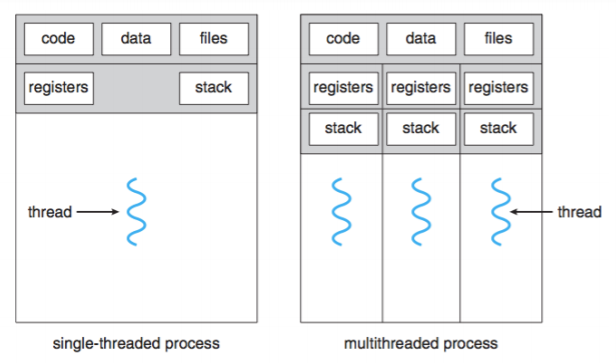
\includegraphics[width=12cm]{unit-14/figures/multithreading.png}
  \caption*{Single and multithreaded processes.}
\end{figure}

Most applications are multithreaded.
Applications are suitable for threading if they need several threads of control.
Examples include web browsers with separate threads for each tab, extension or native utility, as well as any GUI application, so that user events can still be handled while the main thread is performing a computation.

Multithreading is also used in systems that provide services, such as web servers and databases.
When the server receives a request, a new thread is created to service the request, while the main thread continues to listen for new requests.

Threads improve responsiveness, resource sharing and economy --- multithreading results in a smaller memory footprint and greater efficiency of switching between threads.
Threads also improve scalability by enabling the use of parallel processing in multithreaded processors.
They also reduce program complexity by breaking problems into smaller, independent tasks that can execute in parallel.

A system is parallel if it can perform more than one task simultaneously.
A concurrent system supports more than one task by allowing each task to make progress.
Concurrency can be achieved without parallelism.

\subsection{Multicore Systems and Multithreading}

Amdahl's law describes the ratio of performance of a process running on a single processor to the process running on multiple processors in terms of the proportion \(f\) of code that is parallelisable and the number \(N\) of parallel processors.
This ratio is known as `speedup'.
The difference \(\left(1 - f\right)\) is the proportion of the code that is inherently serial.

\begin{equation*}
  \text{speedup} = \frac{\text{time to execute on a single processor}}{\text{time to execute on \(N\) parallel processors}} = \frac{1}{\left(1 - f\right) + \frac{f}{N}}
\end{equation*}

Even a small amount of serial code has a noticeable impact on the overall performance.
There are also overheads to parallelism that are not considered by Amdahl's law.
latency is introduced due to memory access and cache load, for example.

Parallel program introduces a number of challenges.
Pressure is placed on system designers to make better use of multiple cores and to write scheduling algorithms that allow parallel execution.
It is difficult both to modify existing programs and to design new programs to make use of multithreading.
This involves identifying tasks that can be divided in separate, concurrent and, ideally, independent tasks, balancing tasks to achieve efficiency, splitting data and identifying data dependencies.
It is also difficult to test and debug parallel execution since it is non-deterministic.

\subsection{Multithreading Models}

Threads are used through a thread library that exists on the OS or virtual machine.
Operating systems and programming languages provide APIs for creating and managing threads.

Threads may exist at either the user or kernel levels.
user threads are managed above the kernel.
Kernel threads are managed by the OS directly.
Threads can be mapped to processes using three models.

\subsubsection{Many-to-One Model}

The many-to-one model maps many user-level threads to one kernel thread.
Thread management is handled by the thread library in user space, so it is efficient.
However, only one thread can access the kernel at a time since a system call blocks other threads.
This model lacks parallelism on multicore systems and is, therefore, not widely used.

\subsubsection{One-to-One Model}

The one-to-one model maps each user thread to a kernel thread.
This overcomes the issue of blocking, and improves concurrency and parallelism.
However, for each user thread, there must be a kernel thread.

\subsubsection{Many-to-Many Model}

A software developer can create as many user threads as necessary in a thread pool.
Corresponding kernel threads can run in parallel on a multiprocessor.
If a thread blocks, the kernel can schedule another thread for execution.

\subsection{Thread Interference and Memory Consistency}

Threads communicate by sharing data.
If multiple threads reference the same object, thread interference can occur.
This happens when two functions operating on the same data interleave.
This is unpredictable and difficult to debug.

Memory consistency errors occur when different threads have inconsistent views of the same data.
This can be solved through synchronisation, which creates a happens-before relationship between methods and statements.
This guarantees that memory writes by one statement are visible to another.

Two invocations of a synchronised method on the same object cannot be interleaved.
All other threads are blocked until the synchronised thread is complete.
When a synchronised method exits, it automatically establishes a happens-before relationship with any subsequent invocation of a synchronised method on the same object.

Synchronisation is based on intrinsic locks.
These enforce exclusive access and establish happens-before relationships.
Threads must acquire locks before they can do anything.
